\section{Kinematika}
\subsection*{Ponovitev}
\begin{itemize}
    \item \textbf{Kosinusni izrek.} \(c^2 = a^2 + b^2 - 2ab \cos \alpha\), kjer je \(\alpha\) kot med stranicama \(a\) in \(b\).
\end{itemize}

\subsection{Premo gibanje}
\begin{itemize}
    \item \textbf{Enakomerno pospešeno gibanje.} 
    \begin{itemize}
        \item \(a := \frac{dv}{dt} = \text{const}\)
        \item \(\ds dv = a \, dt \lthen \int_{v_0}^{v} \, dv = a \int_{0}^{t} \, dt \lthen v - v_0 = at \lthen  \boxed{v = v_0 + at}\)
        \item \(\ds v := \frac{ds}{dt} \lthen ds = (v_0 + at) \, dt \lthen \int_{0}^{s} \, ds = \int_{0}^{t} (v_0 + at) \, dt \lthen \boxed{s = v_0t + \frac{1}{2}at^2}\)
        \item \(\ds v = \frac{ds}{dt}, \ a = \frac{dv}{dt} \lthen v \, dt = ds, \ a \, dt = dv \lthen \frac{v}{a} = \frac{ds}{dv} \lthen v \, dv = a \, ds \lthen \int_{v_0}^{v} v \, dv = \int_{0}^{s} a \, ds\)
        
        \(\ds \lthen \frac{v^2}{2} - \frac{v_0^2}{2} = as \lthen \boxed{v^2 - v_0^2 = 2as}\), če imamo delo z pojemkom, spremenimo predznak
    \end{itemize}
    \item \textbf{Enakomerno gibanje.} Vzemimo \(a = 0\)
    \item Če se da, izognemo se kvadratnih enačb
    \item \textbf{Prosti pad.} (\(v_0 = 0, \  g = 9.8 \  \text{m} / \text{s}^2\))
    \begin{itemize}
        \item \(\ds \boxed{v = gt, \ t = \sqrt{\frac{2h}{g}}, \ h = \frac{1}{2} g t^2}\)
    \end{itemize}
\end{itemize}

\subsection{Ravninsko gibanje}
\begin{itemize}
    \item \textbf{Relativna hitrost.} \(\vec{v}_r = \vec{v}_1 - \vec{v}_2, \ v_r = |\vec{v}_1 - \vec{v}_2|\)
    
    \item \textbf{Vodoravni met.}
    \begin{center}
        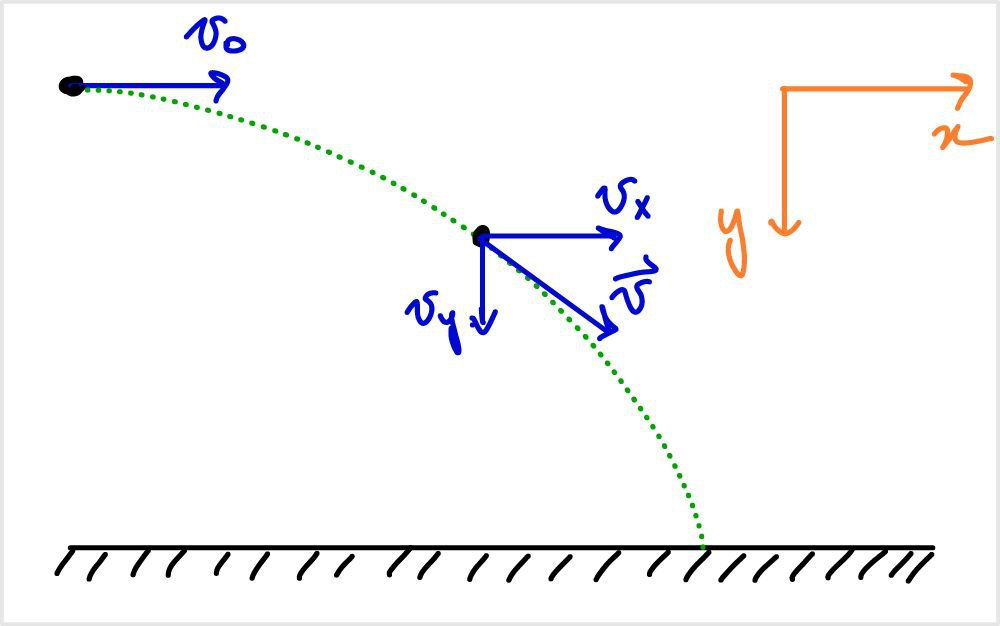
\includegraphics[width=0.35\textwidth]{img/01_001.jpg}      
    \end{center}
    \begin{itemize}
        \item \(\boxed{x(t) = v_0 t, \ y(t) = \frac{1}{2}gt^2}\)
    \end{itemize}
    
    \item \textbf{Poševni met.}
    \begin{center}
        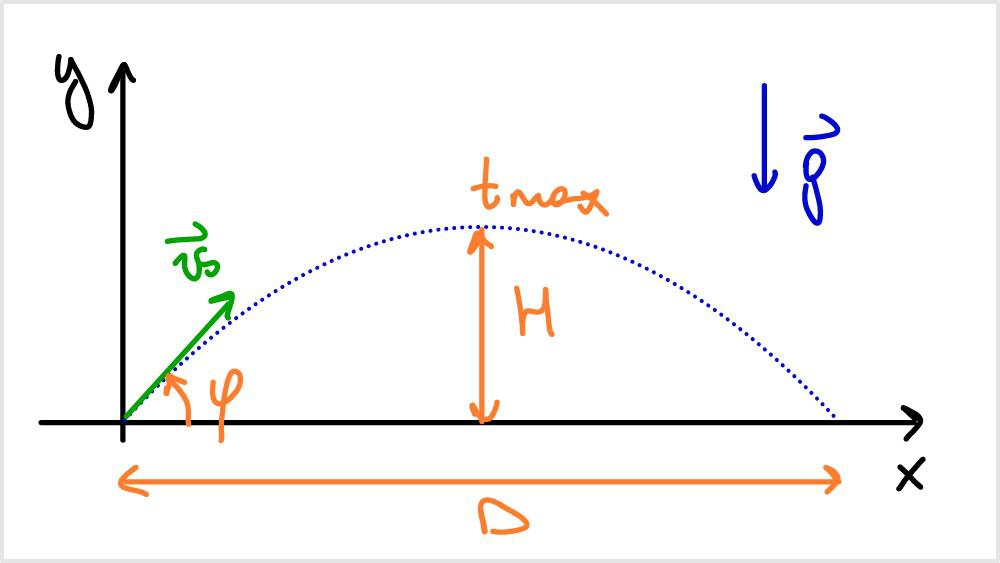
\includegraphics[width=0.35\textwidth]{img/01_002.jpg}      
    \end{center}
    \begin{itemize}
        \item \(\boxed{x(t) = v_0 t \cos \phi, \ y(t) = v_0 t \sin \phi - \frac{1}{2}gt^2}\)
        \item \(\boxed{t_\text{max} = \frac{v_0 \sin \phi}{g}, \ D = \frac{v_0^2 \sin 2 \phi}{g}, \ H = \frac{v_0^2\sin^2 \phi}{2g}}\)
    \end{itemize}
\end{itemize}

